\documentclass[a4paper,12pt]{ctexrep}

% Packages
\usepackage{geometry}
\geometry{left=2.5cm,right=2.5cm,top=3cm,bottom=2.5cm}
\usepackage{graphicx}
\usepackage{float}
\usepackage{listings}
\usepackage{xcolor}
\usepackage{booktabs}
\usepackage{longtable}
\usepackage{hyperref}
\usepackage{fancyhdr}
\usepackage{amsmath}
\usepackage{caption}
\usepackage{subcaption}

% Path to images
\graphicspath{{../img/}}

% Hyperref setup
\hypersetup{
    colorlinks=true,
    linkcolor=black,
    filecolor=magenta,      
    urlcolor=blue,
    pdftitle={Edu Online Education Platform Report},
    pdfpagemode=FullScreen,
}

% Code listing style (Catppuccin Latte inspired)
\definecolor{codegreen}{rgb}{0.25,0.63,0.44}
\definecolor{codegray}{rgb}{0.5,0.5,0.5}
\definecolor{codepurple}{rgb}{0.58,0,0.82}
\definecolor{backcolour}{rgb}{0.95,0.95,0.92}

\lstdefinestyle{mystyle}{
    backgroundcolor=\color{backcolour},   
    commentstyle=\color{codegreen},
    keywordstyle=\color{magenta},
    numberstyle=\tiny\color{codegray},
    stringstyle=\color{codepurple},
    basicstyle=\ttfamily\footnotesize,
    breakatwhitespace=false,         
    breaklines=true,                 
    captionpos=b,                    
    keepspaces=true,                 
    numbers=left,                    
    numbersep=5pt,                  
    showspaces=false,                
    showstringspaces=false,
    showtabs=false,                  
    tabsize=2
}

\lstdefinelanguage{JavaScript}{
  keywords={typeof, new, true, false, catch, function, return, null, catch, switch, var, if, in, while, do, else, case, break, const, let, async, await, try, throw},
  keywordstyle=\color{blue}\bfseries,
  ndkeywords={class, export, boolean, throw, implements, import, this},
  ndkeywordstyle=\color{darkgray}\bfseries,
  identifierstyle=\color{black},
  sensitive=false,
  comment=[l]{//},
  morecomment=[s]{/*}{*/},
  commentstyle=\color{purple}\ttfamily,
  stringstyle=\color{red}\ttfamily,
  morestring=[b]',
  morestring=[b]"
}

\lstset{style=mystyle}

% Header and Footer
\setlength{\headheight}{15pt}
\pagestyle{fancy}
\fancyhf{}
\fancyhead[L]{广州大学课程设计报告}
\fancyhead[R]{Edu-Hub}
\fancyfoot[C]{\thepage}

\begin{document}

% Title Page
\begin{titlepage}
    \centering
    \vspace*{1cm}
    
    \Huge
    \textbf{广州大学课程设计报告}
    
    \vspace{3cm}
    
    \Large
    \renewcommand{\arraystretch}{2.0}
    \begin{tabular}{rc}
        \textbf{系统名称} & \underline{\makebox[9cm][c]{Edu-Hub在线教育平台}} \\
        \textbf{开课学院} & \underline{\makebox[9cm][c]{计算机科学与网络工程学院}} \\
        \textbf{实验室} & \underline{\makebox[9cm][c]{电子信息楼518}} \\
        \textbf{指导教师} & \underline{\makebox[9cm][c]{张少宏、颜国风}} \\
        \textbf{开课时间} & \underline{\makebox[9cm][c]{2025年12月22日-2026年1月3日}} \\
    \end{tabular}

    \vfill
    
    \Large
    \textbf{组员分工表}
    
    \vspace{0.5cm}
    
    \begin{table}[h]
        \centering
        \small
        \renewcommand{\arraystretch}{1.5}
        \setlength{\tabcolsep}{4pt}
        \begin{tabular}{|c|c|c|p{3cm}|p{4.5cm}|c|c|}
            \hline
            \textbf{学号} & \textbf{姓名} & \textbf{班级} & \textbf{项目角色} & \textbf{业务分工} & \textbf{评语} & \textbf{成绩} \\
            \hline
            32306300071 & 杨竣淇 & 软件233 & 
            组长、系统分析师、架构师、测试员 & 
            需求分析、系统设计、前后端开发、数据库设计、接口测试、性能测试 & & \\
            \hline
        \end{tabular}
    \end{table}
    
    \vspace*{1cm}
    
\end{titlepage}

% Table of Contents
\tableofcontents
\newpage



% Real Content Starts Here
\chapter{背景}
\begin{quote}
随着信息技术的飞速发展,“互联网+教育”已成为推动教育现代化的重要引擎。本项目旨在构建一个名为“Edu-Hub”的在线教育平台,利用现代Web技术打破传统教育的时空限制,提供高效、互动的学习体验。
\end{quote}

\section{课题背景}
在数字化转型的浪潮下,传统课堂教学模式正面临着前所未有的挑战与机遇。一方面,优质教育资源的分布不均限制了部分地区学生的学习机会;另一方面,传统的单向灌输式教学难以满足学生个性化、自主化的学习需求。国家《教育信息化2.0行动计划》明确提出要构建“互联网+”条件下的人才培养新模式。在此背景下,开发一款功能完善、交互性强、易于扩展的在线教育平台(Edu-Hub)显得尤为重要。它不仅是技术应用的实践,更是对新型教学模式的探索,旨在通过技术手段实现教育资源的优化配置和共享。

\section{国内外现状}
当前,在线教育市场已呈现出蓬勃发展的态势。

\textbf{国外方面}:以Coursera、edX为代表的MOOC平台汇聚了全球顶尖高校的课程资源,技术成熟,用户体验优秀,但往往存在语言障碍、证书费用高昂以及对特定教学场景适配不足的问题。

\textbf{国内方面}:中国大学MOOC、腾讯课堂、网易云课堂等平台发展迅速,覆盖了从K12到职业教育的广泛领域。然而,这些大型平台通常面向大规模公网用户,对于特定学校或机构的私有化部署、定制化教学管理(如特定的班级管理、实验报告提交等)支持不够灵活。此外,部分平台在师生互动、社区氛围营造方面仍有提升空间,学生容易产生“孤独学习”的倦怠感。

\textbf{本课题切入点}:Edu-Hub 平台定位于一个轻量级、高互动性的在线教学系统,专注于解决中小型教学场景下的资源管理、过程追踪和师生互动问题。

\section{课题内容}
基于上述现状,Edu-Hub 在线教育平台致力于解决传统在线学习中“互动缺失”和“监管困难”两大痛点。
本系统主要包含以下核心内容:
\begin{enumerate}
    \item \textbf{构建多角色用户体系}:实现学生、教师、管理员的分级管理与权限控制,确保系统安全有序。
    \item \textbf{全流程课程管理}:支持课程的创建、富文本介绍编辑、章节视频上传与管理,满足多样化的教学资源展示需求。
    \item \textbf{沉浸式学习体验}:开发视频流媒体播放功能,结合章节导航,提供流畅的学习环境。
    \item \textbf{闭环式教学评估}:通过在线测试、题库管理和自动评分系统,实时检验学习效果。(\textit{注:因开发周期限制,本功能暂未实现})
    \item \textbf{活跃的社区互动}:建立课程评论区和问答社区,促进师生、生生之间的交流与协作。
    \item \textbf{数据驱动的教学决策}:利用可视化图表展示学习进度和成绩分布,为教师调整教学策略提供数据支持。(\textit{注:因开发周期限制,本功能暂未实现})
\end{enumerate}

\section{可行性分析}

\subsection{技术可行性分析/技术路线}
本项目采用当前业界主流且成熟的前后端分离技术栈,具有极高的技术可行性:
\begin{enumerate}
    \item \textbf{前端 (Vue.js 3 + Tailwind CSS)}:Vue 3 的组合式 API (Composition API) 提供了优秀的逻辑复用能力和代码组织方式,配合 Vite 构建工具,开发效率极高。Tailwind CSS 提供了原子化的样式类,能快速构建美观且响应式的用户界面。
    \item \textbf{后端 (Node.js + Express)}:Express 是 Node.js 生态中最流行的 Web 框架,轻量灵活,拥有庞大的中间件生态(如 \texttt{jsonwebtoken} 用于鉴权,\texttt{multer} 用于文件上传),非常适合构建 RESTful API。
    \item \textbf{数据库 (MySQL 8.0)}:MySQL 是最流行的开源关系型数据库,支持事务处理和复杂的关联查询,能够稳定存储用户信息、课程结构、学习进度等核心数据。
    \item \textbf{状态管理与交互 (Pinia + Axios)}:Pinia 作为 Vue 的新一代状态管理库,轻量且直观;Axios 则是处理 HTTP 请求的标准库。
\end{enumerate}
综上所述,开发团队对上述技术栈有充分的掌握,且社区资源丰富,遇到问题易于解决,技术风险可控。

\subsection{本课题的意义}
\textbf{社会意义}:Edu-Hub 平台的推广有助于打破地域限制,促进优质教育资源的跨区域流动,在一定程度上缓解教育资源分配不均的问题,促进教育公平。同时,它为终身学习者提供了便捷的渠道,助力学习型社会的建设。

\textbf{经济意义}:对于教育培训机构或学校而言,部署 Edu-Hub 平台可以大幅降低线下教学的场地租赁、纸质资料印刷等成本。通过自动化的作业批改和数据统计,能显著减轻教师的重复性工作负担,提高教学管理的效率和产出比。

\chapter{需求分析}

\section{需求概况}

\subsection{组织机构图与用户分析}
Edu-Hub 平台主要涉及三类用户角色,各角色的职责如下:
\begin{itemize}
    \item \textbf{学生 (Student)}:系统的主要使用者。可以浏览课程列表、选课报名、观看视频教程、参与在线测试、在评论区互动以及查看个人学习进度。
    \item \textbf{教师 (Teacher)}:课程内容的提供者。负责创建和管理课程、上传教学视频、发布考试题目、批改主观题(如有)、回复学生提问以及查看班级学习数据。
    \item \textbf{管理员 (Administrator)}:系统的维护者。拥有最高权限,负责用户账号管理(如封禁违规用户)、全站课程审核、系统配置以及数据备份。
\end{itemize}

\subsection{主体业务需求}
Edu-Hub 平台的核心业务流程围绕“教”与“学”展开,具体需求如下:
\begin{enumerate}
    \item \textbf{用户管理业务}:学生用户仅需提供用户名和密码即可完成注册。登录时,后端验证账号密码并颁发 JWT 令牌。前端根据令牌中的角色字段(Role)动态渲染菜单权限。
    \item \textbf{课程管理业务}:教师在后台创建课程,填写标题、简介(富文本),并上传封面图。课程创建后,教师可添加章节,每个章节支持上传视频文件。视频上传后需经服务器处理存储。
    \item \textbf{视频学习业务}:学生进入课程详情页,点击章节视频进行播放。系统需记录播放进度,支持断点续播。
    \item \textbf{在线测试业务}:教师在题库中添加题目(单选、多选、判断),并组卷发布。学生在规定时间内答题,提交后系统自动比对答案并计算客观题得分。(\textit{注:部分功能待完善})
    \item \textbf{社区互动业务}:每个课程下方设有评论区,学生可发表疑问或心得,教师和其他学生可进行回复。支持即时显示新消息。
    \item \textbf{数据分析业务}:系统自动采集学生的学习行为(视频观看时长、测试成绩),通过可视化图表(如柱状图、饼图)向教师展示课程的及格率、活跃度等指标。(\textit{注:部分功能待完善})
\end{enumerate}

\textbf{注意:安全需求是业务需求的一部分。}

\subsection{质量需求}
质量需求表现为软件满足预期的程度:
\begin{itemize}
    \item \textbf{性能需求}:
    \begin{itemize}
        \item 视频首屏加载时间不超过 2 秒(在正常网络环境下)。
        \item 系统支持至少 100 人同时在线并发访问而不崩溃。
        \item API 接口平均响应时间低于 500ms。
    \end{itemize}
    \item \textbf{安全性需求}:
    \begin{itemize}
        \item 所有敏感数据(如密码)需经过哈希加盐存储 [TODO: 待实现]。
        \item API 接口需进行 JWT 身份验证,防止未授权访问。
        \item 文件上传需校验格式和大小,防止恶意脚本注入。
    \end{itemize}
    \item \textbf{可靠性需求}:
    \begin{itemize}
        \item 系统应具备 99.9\% 的可用性。
        \item 关键数据(如成绩、课程进度)需定期自动备份。
    \end{itemize}
\end{itemize}

\textbf{注意:性能需求是质量需求的一部分。}

\subsection{其它(约束性)需求}
指软件开发过程、运行环境应满足的(非业务)约束:
\begin{itemize}
    \item \textbf{开发周期}:本项目需在课程设计规定的 2 周时间内完成开发与测试。
    \item \textbf{技术约束}:前端必须使用 Vue.js 3 + Tailwind CSS,后端采用 Node.js (Express) + MySQL 8.0。
    \item \textbf{运行环境}:服务端需部署在 Linux/Windows 服务器上,客户端需支持主流浏览器(Chrome, Edge, Firefox)。
\end{itemize}

\textbf{注意:通常把接口需求单独列为一类需求。}

\section{用例分析(功能需求详细分析)}
本系统主要包含学生、教师、管理员三类角色。根据业务需求分析,各角色的核心用例设计如下。

\subsection{学生用例视图}
学生是系统的主要使用者,其核心需求围绕“课程学习”与“社区互动”展开。

\begin{figure}[H]
    \centering
    \includegraphics[width=0.9\textwidth, page=1]{Student.pdf}
    \caption{学生用例图}
    \label{fig:student_usecase}
\end{figure}

主要用例包括:
\begin{enumerate}
    \item \textbf{用户系统}:登录/注册、个人信息管理(修改头像/密码)。
    \item \textbf{课程系统}:
    \begin{itemize}
        \item \textbf{选课前}:浏览开放课程、搜索课程 [待完善]、选修课程。
        \item \textbf{选课后}:查看我的课程、观看视频、参加考试 [待完善]、查看得分。
    \end{itemize}
    \item \textbf{论坛系统}:浏览论坛、发表帖子(关联课程/章节)、回复帖子。
\end{enumerate}

\subsection{教师用例视图}
教师是教学资源的生产者,负责课程的建设与维护。

\begin{figure}[H]
    \centering
    \includegraphics[width=0.9\textwidth, page=1]{Teacher.pdf}
    \caption{教师用例图}
    \label{fig:teacher_usecase}
\end{figure}

主要用例包括:
\begin{enumerate}
    \item \textbf{用户系统}:注册(需邀请码)、登录、个人信息管理。
    \item \textbf{教学管理}:
    \begin{itemize}
        \item \textbf{课程生产}:查看已创建课程列表、创建/发布课程、编辑课程信息、管理章节(支持三级目录)、上传视频/课件。
        \item \textbf{课程维护}:下架/上架课程 [下架功能待完善]。
        \item \textbf{数据查看}:查看学生成绩统计 [待完善]。
    \end{itemize}
    \item \textbf{互动管理}:在课程后台直接查看并回复关联的帖子。
\end{enumerate}

\subsection{管理员用例视图}
管理员负责系统的整体运维与监管。

\begin{figure}[H]
    \centering
    \includegraphics[width=0.9\textwidth, page=1]{Admin.pdf}
    \caption{管理员用例图}
    \label{fig:admin_usecase}
\end{figure}

主要用例包括:
\begin{enumerate}
    \item \textbf{账号管理}:生成教师邀请码、查看/搜索用户列表、封禁/解封违规账号、重置用户密码。
    \item \textbf{内容监管}:全局课程管理 [待完善]、封禁违规课程 [待完善]。
    \item \textbf{个人中心}:修改管理员自身密码 [待完善]。
\end{enumerate}

\begin{quote}
此后需求分析部分分别对各用例展开详尽的描述。
\end{quote}

\section{用户注册与登录}
本用例描述用户(学生、教师、管理员)进入系统并获取身份授权的过程。

\subsection{用例中的类}
参与类包括:\texttt{User} (用户实体), \texttt{InviteCode} (邀请码实体), \texttt{AuthController} (认证控制器)。

\subsection{关键的类及状态}
\begin{itemize}
    \item \textbf{User}: 状态包括 \texttt{ACTIVE} (活跃), \texttt{BANNED} (封禁)。
    \item \textbf{InviteCode}: 状态包括 \texttt{USED} (已使用), \texttt{UNUSED} (未使用)。
\end{itemize}

\subsection{用例主体行为}
\begin{enumerate}
    \item \textbf{进入页面}:用户访问系统首页,点击“登录”或“注册”。
    \item \textbf{提交信息}:
    \begin{itemize}
        \item \textbf{注册}:输入用户名、密码、昵称。(教师角色需输入有效邀请码)。
        \item \textbf{登录}:输入用户名、密码。
    \end{itemize}
    \item \textbf{后端验证}:
    \begin{itemize}
        \item 系统校验用户名是否唯一。
        \item 系统校验密码正确性(注册时校验格式,登录时校验匹配)。
        \item (仅教师注册)系统校验邀请码是否存在且未过期。
    \end{itemize}
    \item \textbf{授权响应}:验证通过后,服务器生成 JWT Token 并返回给客户端。
    \item \textbf{跳转}:前端将 Token 存入 LocalStorage,并根据用户角色(Role)跳转至相应 Dashboard。
\end{enumerate}

\subsection{用例异常行为}
\begin{itemize}
    \item \textbf{用户名已存在}:注册时提示“用户名已被占用”。
    \item \textbf{邀请码无效}:教师注册时提示“邀请码无效或已过期”。
    \item \textbf{凭据错误}:登录时提示“用户名或密码错误”。
\end{itemize}

\section{课程发布与管理}
本用例描述教师创建新课程并发布内容的完整流程。

\subsection{用例中的类}
参与类包括:\texttt{Course} (课程), \texttt{Chapter} (章节), \texttt{User} (教师)。

\subsection{关键的类及状态}
\begin{itemize}
    \item \textbf{Course}: 状态流转:\texttt{DRAFT} (草稿) $\rightarrow$ \texttt{PUBLISHED} (已发布)。只有 \texttt{PUBLISHED} 状态的课程对学生可见。
\end{itemize}

\subsection{用例主体行为}
\begin{enumerate}
    \item \textbf{创建课程}:教师点击“新建课程”,填写标题、简介、上传封面图,设置课程类型(公开/私有)。
    \item \textbf{构建大纲}:教师添加章节(Chapter),支持多级目录结构。
    \item \textbf{上传资源}:教师在章节下上传教学视频文件。
    \item \textbf{发布课程}:教师确认课程内容无误后,点击“发布”按钮。
    \item \textbf{系统处理}:系统将课程状态更新为 \texttt{PUBLISHED},并在课程大厅展示。
\end{enumerate}

\subsection{用例异常行为}
\begin{itemize}
    \item \textbf{空章节发布}:若课程内无任何章节,系统阻止发布并提示“请至少添加一个章节”。
    \item \textbf{上传失败}:若视频文件格式不支持或过大,系统提示上传失败。
\end{itemize}

\section{视频学习}
本用例描述学生进入课程并观看教学视频的学习过程。

\subsection{用例中的类}
参与类包括:\texttt{Enrollment} (选课记录), \texttt{ChapterProgress} (章节进度), \texttt{Course} (课程)。

\subsection{关键的类及状态}
\begin{itemize}
    \item \textbf{ChapterProgress}: 记录用户的观看进度(\texttt{progress})和完成状态(\texttt{is\_completed})。
\end{itemize}

\subsection{用例主体行为}
\begin{enumerate}
    \item \textbf{进入课程}:学生在“我的课程”列表中点击进入课程详情页。
    \item \textbf{选择章节}:在左侧章节树中点击带有视频标识的节点。
    \item \textbf{播放视频}:系统加载视频播放器,自动跳转至上次观看的断点。
    \item \textbf{进度同步}:播放过程中,前端定时向后端发送心跳包,更新 \texttt{ChapterProgress}。
    \item \textbf{完成学习}:视频播放结束,系统自动标记该章节为“已完成”。
\end{enumerate}

\subsection{用例异常行为}
\begin{itemize}
    \item \textbf{未选课访问}:若用户未选修该课程,系统拒绝访问视频并提示“请先加入课程”。
\end{itemize}

\section{社区互动}
本用例描述用户在课程讨论区发表观点和互动的过程。

\subsection{用例中的类}
参与类包括:\texttt{Post} (帖子), \texttt{Comment} (评论), \texttt{User} (作者)。

\subsection{关键的类及状态}
\begin{itemize}
    \item \textbf{Post}: 关联特定的 \texttt{Course} 或 \texttt{Chapter}。
\end{itemize}

\subsection{用例主体行为}
\begin{enumerate}
    \item \textbf{浏览帖子}:用户进入课程讨论区,查看帖子列表。
    \item \textbf{发表帖子}:用户点击“发帖”,输入标题和内容,点击提交。
    \item \textbf{回复互动}:用户进入帖子详情,在底部输入框填写评论并提交。
    \item \textbf{展示更新}:列表自动刷新,显示最新的帖子和评论。
\end{enumerate}

\subsection{用例异常行为}
\begin{itemize}
    \item \textbf{内容违规}:(预留) 若包含敏感词,系统拦截发布。
\end{itemize}

\section{完整的类图}
\begin{figure}[H]
    \centering
    \includegraphics[width=0.9\textwidth, page=1]{Class.pdf}
    \caption{系统完整类图}
    \label{fig:class_diagram}
\end{figure}

\section{用户验收测试计划}
按照W模型的观点,在需求分析结束时,应及时规划测试工程,并展开对测试需求的分析,设计确认(用户验收)测试的流程、数据(用例)等。
\begin{quote}
在行文时,可归并到单独的测试章节。
\end{quote}

\chapter{概要设计}

本系统采用经典的前后端分离架构(B/S模式),前端基于 Vue.js 3 生态构建单页应用(SPA),后端基于 Node.js (Express) 提供 RESTful API 服务,数据库采用 MySQL 8.0。这种架构实现了视图层与业务逻辑层的完全解耦,便于团队并行开发与后期维护。

\section{系统分解(体系结构)}

系统整体架构分为三个主要层次:表现层(Frontend)、业务逻辑层(Backend)和数据持久层(Database)。

\subsection{架构图}
\begin{figure}[H]
    \centering
    \includegraphics[width=0.95\textwidth, height=0.8\textheight, keepaspectratio]{Architecture.pdf}
    \caption{系统架构图}
    \label{fig:architecture}
\end{figure}

\subsection{子系统职责定义}

\begin{enumerate}
    \item \textbf{前端子系统 (\texttt{frontend/})}
    \begin{itemize}
        \item \textbf{视图层 (\texttt{views/})}:负责页面的结构展示。核心模块包括 \texttt{auth} (认证)、\texttt{course} (课程展示)、\texttt{dashboard} (后台管理)。
        \item \textbf{组件层 (\texttt{components/})}:封装可复用的 UI 元素,如 \texttt{ChapterEditor.vue} (章节编辑器) 和通用布局组件。
        \item \textbf{状态管理 (\texttt{stores/})}:使用 Pinia 管理全局状态。例如 \texttt{auth.js} 存储用户信息和 JWT Token,\texttt{course.js} 缓存课程列表数据。
        \item \textbf{网络层 (\texttt{utils/request.js})}:基于 Axios 封装 HTTP 请求,统一处理请求拦截(注入 Token)和响应拦截(错误处理)。
    \end{itemize}

    \item \textbf{后端子系统 (\texttt{backend/})}
    \begin{itemize}
        \item \textbf{接口层 (\texttt{routes/})}:定义 API 路由端点。例如 \texttt{authRoutes.js} 处理登录注册,\texttt{courseRoutes.js} 处理课程增删改查。
        \item \textbf{业务层 (\texttt{controllers/})}:实现核心业务逻辑。例如 \texttt{courseController.js} 负责解析上传的视频文件、验证数据完整性并调用模型。
        \item \textbf{中间件 (\texttt{middleware/})}:\texttt{authMiddleware.js} 负责解析 HTTP Header 中的 JWT 令牌,验证用户身份并拦截非法请求。
        \item \textbf{数据层 (\texttt{models/})}:使用 Sequelize 定义数据模型(Schema),如 \texttt{User.js}, \texttt{Course.js},自动映射到 MySQL 表结构。
    \end{itemize}

    \item \textbf{数据存储子系统}
    \begin{itemize}
        \item \textbf{MySQL}:存储结构化数据(用户、课程元数据、评论等)。
        \item \textbf{本地文件系统 (\texttt{uploads/})}:存储非结构化数据(用户头像、课程封面、教学视频),通过 Express 的静态资源中间件对外提供访问。
    \end{itemize}
\end{enumerate}

\section{系统总体流程}

本系统采用 RESTful 风格进行通信。以下以“教师发布课程”为例,描述跨子系统的数据流转过程(采用\textbf{异步上传}模式):

\begin{enumerate}
    \item \textbf{封面上传}:教师在前端选择封面图片,组件调用通用上传接口 \texttt{POST /api/upload}。
    \begin{itemize}
        \item 后端 \texttt{uploadController} 接收文件流,保存至 \texttt{backend/uploads/},并返回文件访问 URL。
    \end{itemize}
    \item \textbf{发起建课请求}:教师填写课程信息(包含上一步获取的封面 URL),点击发布。Vue 组件调用 \texttt{courseStore.createCourse()}。
    \item \textbf{网络传输}:Axios 拦截请求,在 Header 中添加 \texttt{Authorization: Bearer <token>},并将课程数据封装为 \textbf{JSON} 格式发送至 \texttt{POST /api/courses}。
    \item \textbf{路由分发}:Express 接收请求,\texttt{authMiddleware} 验证 Token 有效性。若通过,将请求转发至 \texttt{courseController.createCourse}。
    \item \textbf{业务处理}:
    \begin{itemize}
        \item Controller 从 \texttt{req.body} 中提取 \texttt{title}, \texttt{description}, \texttt{cover\_image} (URL) 等字段。
        \item Controller 验证必填字段非空。
        \item Controller 调用 \texttt{Course.create()} 模型方法。
    \end{itemize}
    \item \textbf{数据持久化}:Sequelize 生成 \texttt{INSERT INTO courses ...} SQL 语句并在 MySQL 中执行。
    \item \textbf{响应反馈}:数据库返回新创建的课程对象,后端封装 JSON 响应返回给前端。
    \item \textbf{界面更新}:前端接收响应,Pinia 更新本地课程列表状态,路由跳转至课程管理页。
\end{enumerate}

\section{界面设计原则(交互风格规范)}

前端界面设计遵循“简洁、响应式、组件化”的原则,主要依托 \textbf{Tailwind CSS} 框架实现。

\begin{enumerate}
    \item \textbf{原子化样式}:使用 Tailwind 的原子类(如 \texttt{p-4}, \texttt{flex}, \texttt{text-blue-500})构建样式,确保全站间距、颜色、字体的一致性,避免传统 CSS 的样式冲突。
    \item \textbf{主题定制}:引入 \textbf{Catppuccin} 主题配色方案,为系统提供了一套柔和、低对比度的色彩风格,既美观又护眼,提升了用户的视觉体验。
    \item \textbf{响应式布局}:采用 Mobile-First 策略,利用 \texttt{md:}, \texttt{lg:} 前缀适配不同屏幕尺寸。例如,课程列表在移动端为单列,桌面端自动切换为网格布局。
    \item \textbf{交互反馈}:
    \begin{itemize}
        \item \textbf{加载状态}:数据请求期间展示 Loading 骨架屏或旋转图标。
        \item \textbf{操作反馈}:使用 \texttt{useToast.js} 封装的全局消息组件,在操作成功或失败时在页面顶部弹出自动消失的提示框。
    \end{itemize}
    \item \textbf{组件复用}:将通用的功能模块(如“文件上传区域”、“富文本编辑器容器”)封装为独立组件,保持代码整洁。
\end{enumerate}

\section{界面原型设计}

基于上述设计原则,本系统设计了以下核心界面原型,以直观展示系统的功能布局与交互逻辑。\textit{(说明:因开发时间有限,原型图为低保真的色块区分布局。)}

\subsection{登录与注册页}
\begin{figure}[H]
    \centering
    \begin{subfigure}[b]{0.48\textwidth}
        \includegraphics[width=\textwidth, page=3]{proto/main.pdf}
        \caption{登录页}
    \end{subfigure}
    \hfill
    \begin{subfigure}[b]{0.48\textwidth}
        \includegraphics[width=\textwidth, page=4]{proto/main.pdf}
        \caption{注册页}
    \end{subfigure}
    \caption{认证页面原型}
\end{figure}

\subsection{主页 (Home)}
\begin{figure}[H]
    \centering
    \begin{subfigure}[b]{0.48\textwidth}
        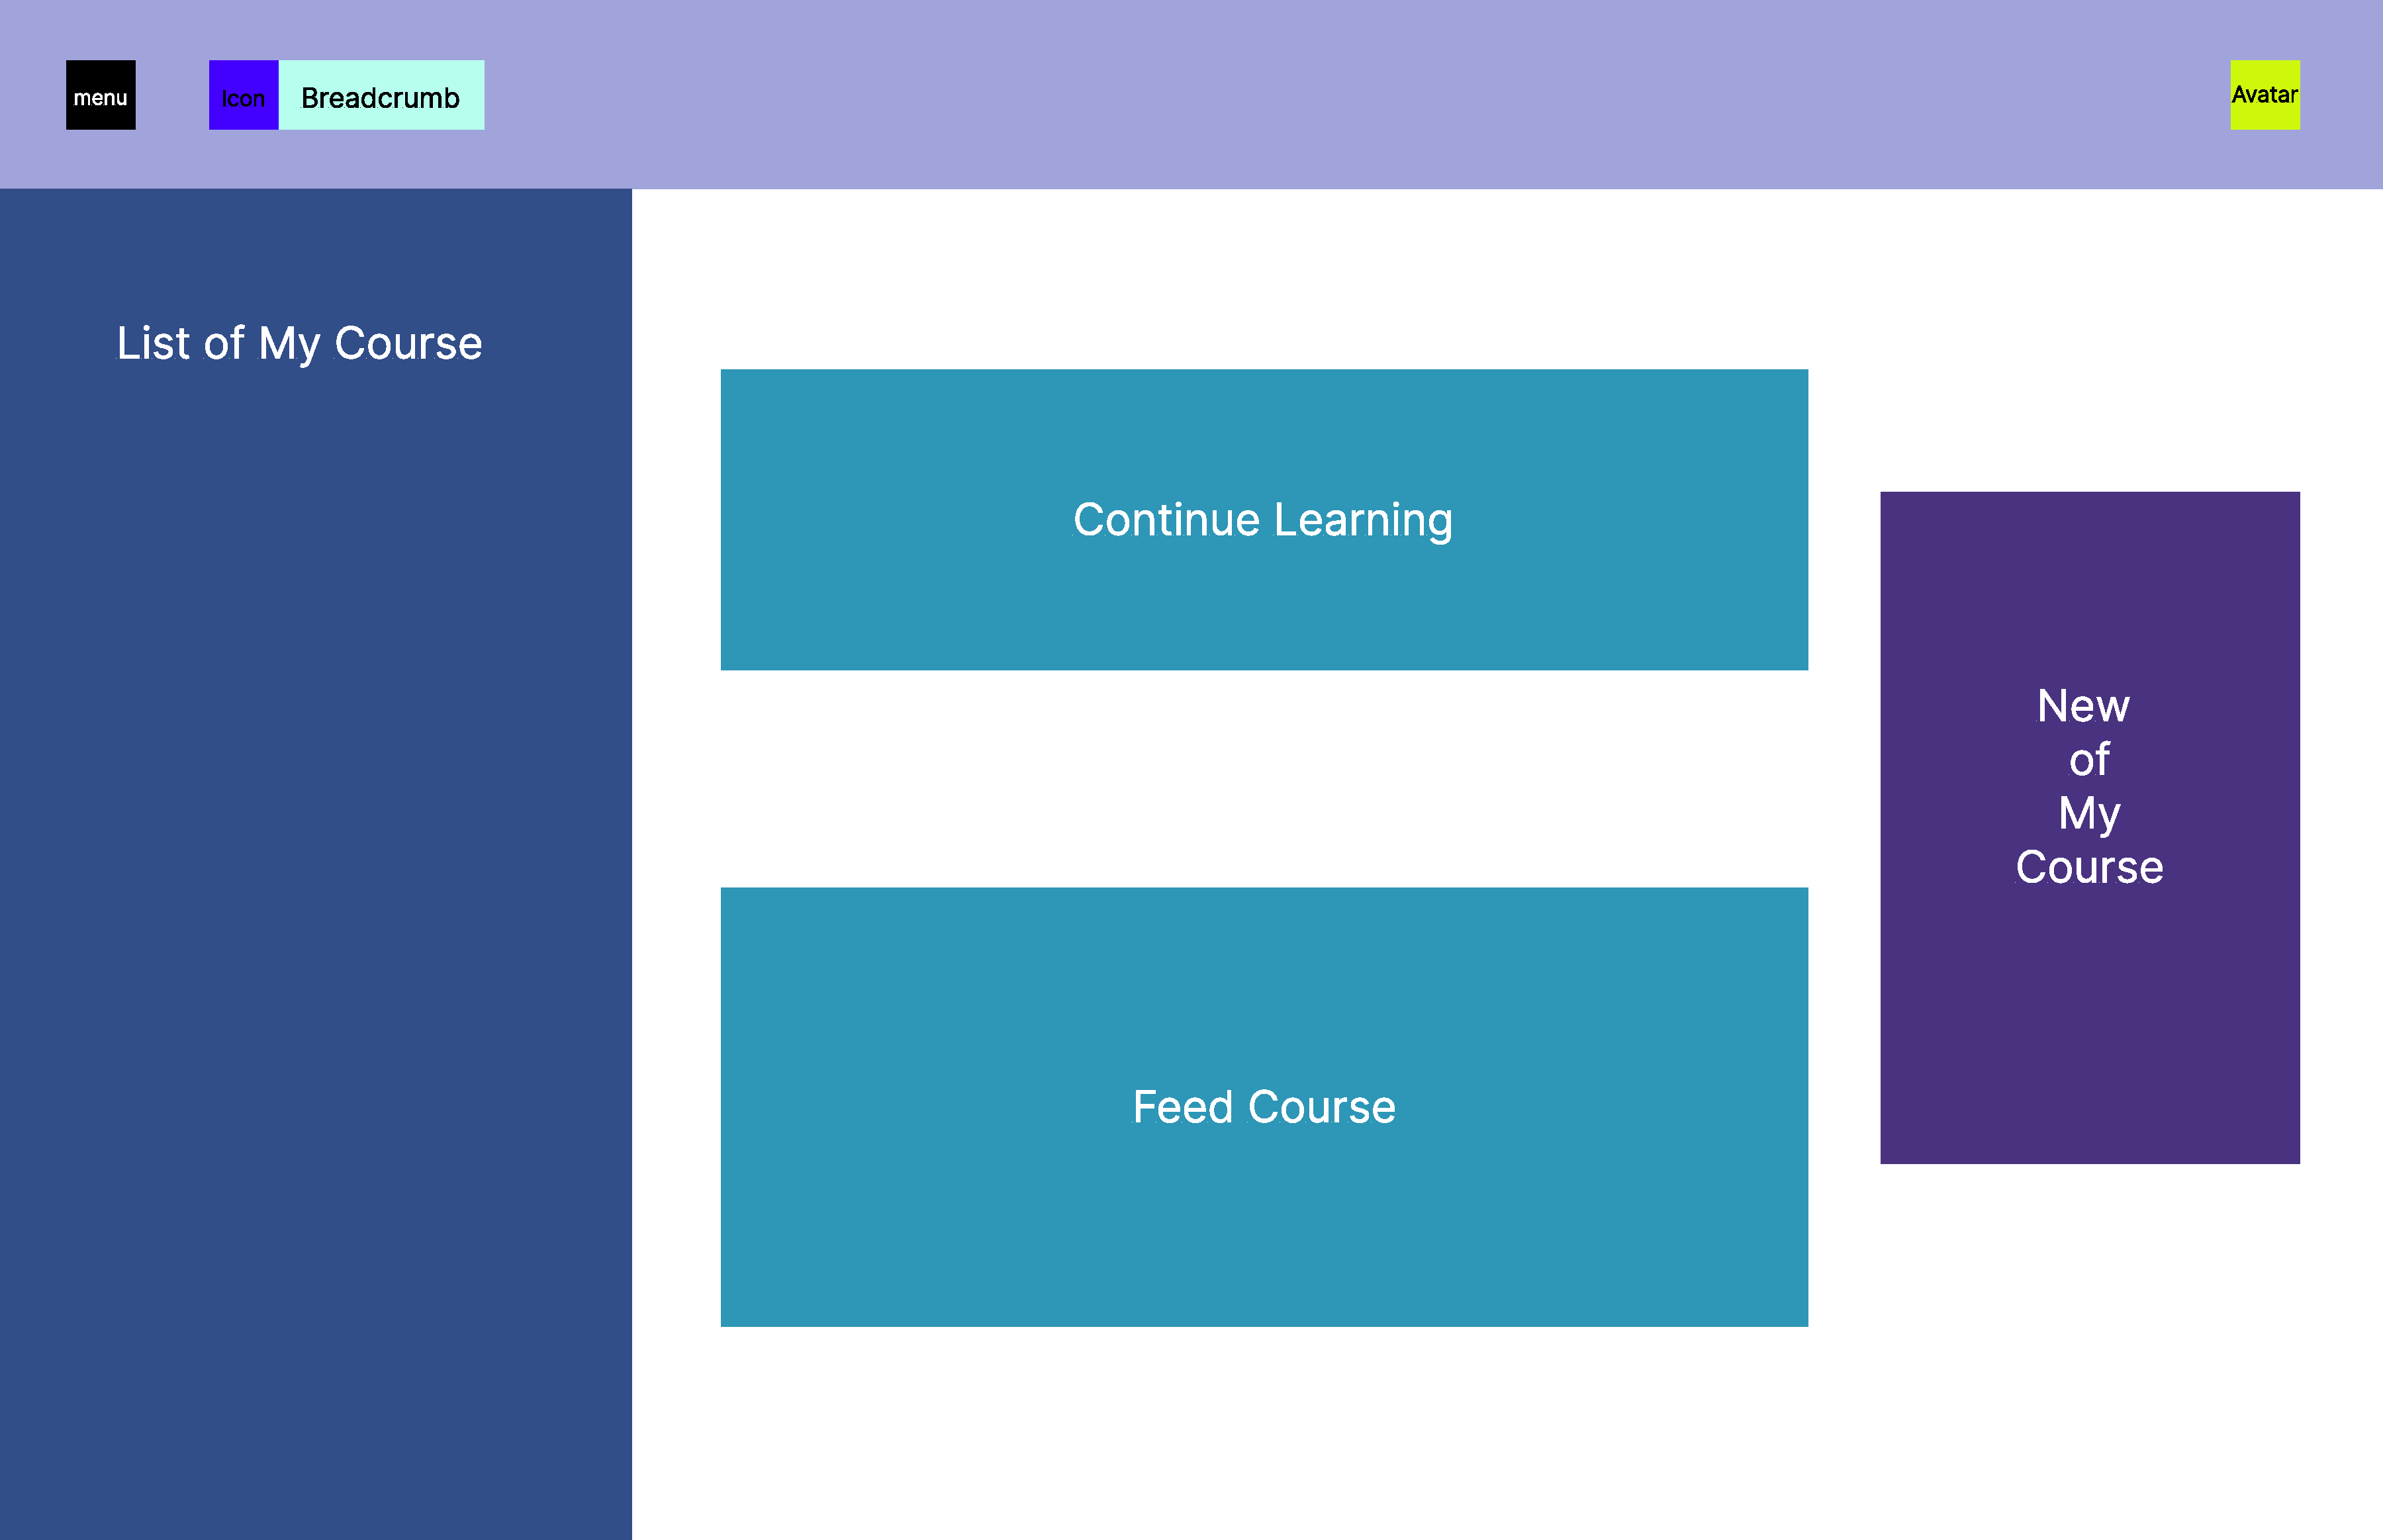
\includegraphics[width=\textwidth, page=1]{proto/main.pdf}
        \caption{主页}
    \end{subfigure}
    \hfill
    \begin{subfigure}[b]{0.48\textwidth}
        \includegraphics[width=\textwidth, page=2]{proto/main.pdf}
        \caption{主页侧边栏展开}
    \end{subfigure}
    \caption{主页原型}
\end{figure}

\subsection{课程广场}
\begin{figure}[H]
    \centering
    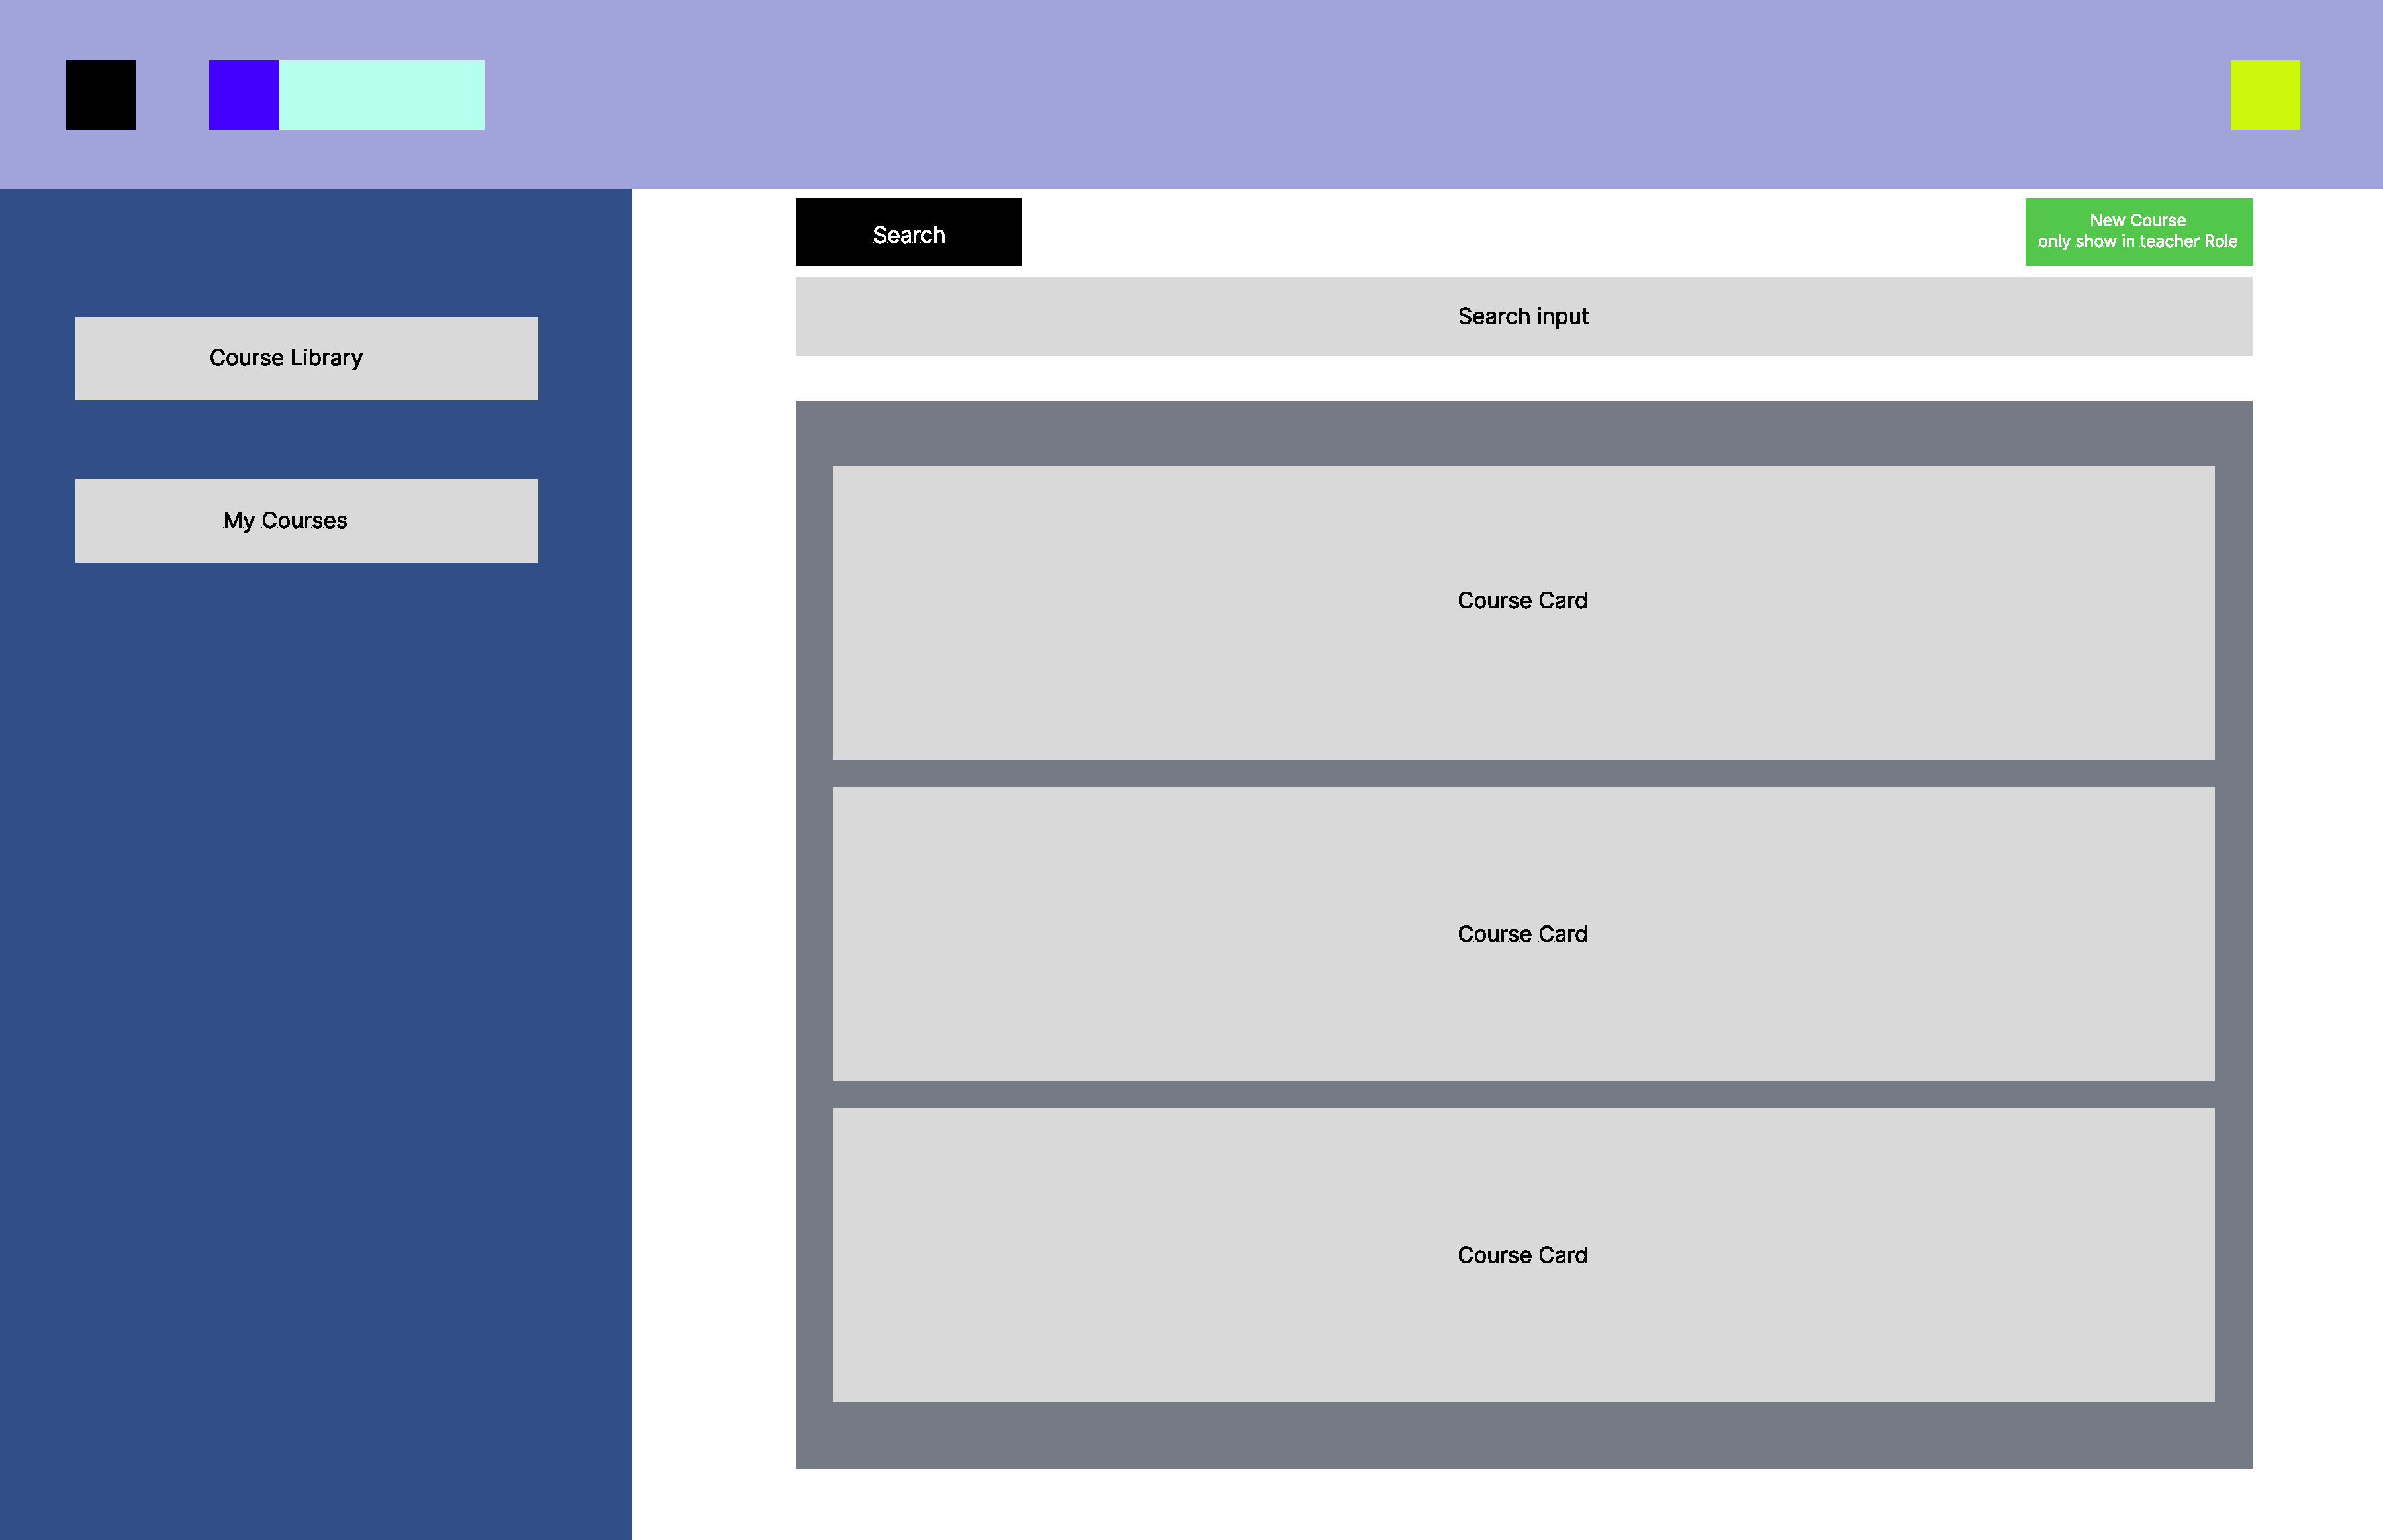
\includegraphics[width=0.8\textwidth, page=1]{proto/course.pdf}
    \caption{课程广场原型}
\end{figure}

\subsection{课程学习页}
\begin{figure}[H]
    \centering
    \includegraphics[width=0.8\textwidth, page=2]{proto/course.pdf}
    \caption{课程学习页原型}
\end{figure}

\subsection{课程编辑器}
\begin{figure}[H]
    \centering
    \includegraphics[width=0.8\textwidth, page=6]{proto/course.pdf}
    \caption{课程编辑器原型}
\end{figure}

\section{系统集成测试计划与设计}

集成测试旨在验证前后端接口的连通性及业务流程的完整性。

\begin{enumerate}
    \item \textbf{接口测试 (API Testing)}
    \begin{itemize}
        \item \textbf{工具}:Apifox。
        \item \textbf{策略}:独立测试后端 API。重点测试 \texttt{authRoutes} 的 Token 生成与验证,以及 \texttt{uploadRoutes} 的文件上传功能(边界条件:文件大小限制、格式限制)。
    \end{itemize}
    \begin{figure}[H]
        \centering
        \includegraphics[width=0.8\textwidth]{apifox.png}
        \caption{Apifox 接口调试示例}
    \end{figure}
    \item \textbf{前后端联调 (Integration)}
    \begin{itemize}
        \item \textbf{环境}:前端运行于 \texttt{localhost:5173},后端运行于 \texttt{localhost:3000}。
        \item \textbf{测试场景}:
        \begin{itemize}
            \item \textbf{注册登录流}:注册新账号 $\rightarrow$ 自动跳转登录 $\rightarrow$ 登录获取 Token $\rightarrow$ 访问受保护的 Dashboard。
            \item \textbf{课程生命周期}:创建课程 $\rightarrow$ 添加章节 $\rightarrow$ 上传视频 $\rightarrow$ 学生选课 $\rightarrow$ 观看视频(进度更新)。
        \end{itemize}
    \end{itemize}
    \item \textbf{异常处理测试}
    \begin{itemize}
        \item 模拟网络断开或后端宕机,验证前端 Axios 拦截器是否能正确捕获错误并提示用户。
        \item 模拟 Token 过期,验证前端是否能自动清除本地存储并跳转至登录页。
    \end{itemize}
\end{enumerate}

\chapter{详细设计}

本章基于实际代码结构(Reverse Engineering)对系统的核心数据模型、关键业务逻辑及算法进行详细描述。

\section{类(数据)设计}

系统采用 Sequelize ORM 框架定义数据模型,底层映射为 MySQL 关系型数据库表。以下为核心物理数据模型设计。

\subsection{数据库物理模型}

系统数据库的实体关系图(ER图)如下图所示,清晰展示了用户、课程、章节、进度、评论等核心实体及其之间的关联关系(如一对多、多对多等)。

\begin{figure}[H]
    \centering
    \includegraphics[width=0.95\textwidth]{DB.pdf}
    \caption{数据库ER图}
    \label{fig:db_er}
\end{figure}

\subsubsection{数据表定义}

% User Table
\begin{longtable}{lllll}
\caption{用户表 (User)} \\
\toprule
\textbf{字段名} & \textbf{类型} & \textbf{必填} & \textbf{默认值} & \textbf{描述} \\
\midrule
\endfirsthead
\toprule
\textbf{字段名} & \textbf{类型} & \textbf{必填} & \textbf{默认值} & \textbf{描述} \\
\midrule
\endhead
\bottomrule
\endfoot
id & INTEGER & 是 & Auto Inc & 主键 \\
username & STRING & 是 & - & 登录账号 (唯一索引) \\
password & STRING & 是 & - & 登录密码 (当前版本暂存明文,建议升级为 Bcrypt 哈希) \\
nickname & STRING & 否 & - & 用户昵称 \\
role & ENUM & 是 & STUDENT & 角色: STUDENT, TEACHER, ADMIN \\
status & ENUM & 是 & ACTIVE & 状态: ACTIVE, BANNED \\
created\_at & DATETIME & 是 & Now & 创建时间 \\
\end{longtable}

% Course Table
\begin{longtable}{lllll}
\caption{课程表 (Course)} \\
\toprule
\textbf{字段名} & \textbf{类型} & \textbf{必填} & \textbf{默认值} & \textbf{描述} \\
\midrule
\endfirsthead
\toprule
\textbf{字段名} & \textbf{类型} & \textbf{必填} & \textbf{默认值} & \textbf{描述} \\
\midrule
\endhead
\bottomrule
\endfoot
id & INTEGER & 是 & Auto Inc & 主键 \\
title & STRING & 是 & - & 课程标题 \\
description & TEXT & 否 & - & 课程简介 \\
cover\_image & STRING & 否 & - & 封面图片 URL \\
type & ENUM & 是 & PUBLIC & 类型: PUBLIC (公开), PRIVATE (私有) \\
status & ENUM & 是 & DRAFT & 状态: DRAFT, PUBLISHED, BANNED \\
teacher\_id & INTEGER & 是 & - & 外键 $\rightarrow$ User.id \\
\end{longtable}

% Chapter Table
\begin{longtable}{lllll}
\caption{章节表 (Chapter)} \\
\toprule
\textbf{字段名} & \textbf{类型} & \textbf{必填} & \textbf{默认值} & \textbf{描述} \\
\midrule
\endfirsthead
\toprule
\textbf{字段名} & \textbf{类型} & \textbf{必填} & \textbf{默认值} & \textbf{描述} \\
\midrule
\endhead
\bottomrule
\endfoot
id & INTEGER & 是 & Auto Inc & 主键 \\
course\_id & INTEGER & 是 & - & 外键 $\rightarrow$ Course.id \\
parent\_id & INTEGER & 否 & NULL & 父章节ID (实现树形结构) \\
title & STRING & 是 & - & 章节标题 \\
type & VIRTUAL & - & - & 逻辑字段: FOLDER (目录) / FILE (内容) \\
video\_url & STRING & 否 & - & 视频文件地址 \\
resource\_url & STRING & 否 & - & 课件下载地址 \\
order & INTEGER & 是 & 0 & 排序权重 \\
\end{longtable}

% ChapterProgress Table
\begin{longtable}{lllll}
\caption{学习进度表 (ChapterProgress)} \\
\toprule
\textbf{字段名} & \textbf{类型} & \textbf{必填} & \textbf{默认值} & \textbf{描述} \\
\midrule
\endfirsthead
\toprule
\textbf{字段名} & \textbf{类型} & \textbf{必填} & \textbf{默认值} & \textbf{描述} \\
\midrule
\endhead
\bottomrule
\endfoot
id & INTEGER & 是 & Auto Inc & 主键 \\
user\_id & INTEGER & 是 & - & 外键 $\rightarrow$ User.id \\
chapter\_id & INTEGER & 是 & - & 外键 $\rightarrow$ Chapter.id \\
course\_id & INTEGER & 是 & - & 外键 $\rightarrow$ Course.id (冗余字段优化查询) \\
progress & INTEGER & 是 & 0 & 观看进度 (0-100) \\
is\_completed & BOOLEAN & 是 & false & 是否完成 \\
\end{longtable}

% Enrollment Table
\begin{longtable}{lllll}
\caption{选课记录表 (Enrollment)} \\
\toprule
\textbf{字段名} & \textbf{类型} & \textbf{必填} & \textbf{默认值} & \textbf{描述} \\
\midrule
\endfirsthead
\toprule
\textbf{字段名} & \textbf{类型} & \textbf{必填} & \textbf{默认值} & \textbf{描述} \\
\midrule
\endhead
\bottomrule
\endfoot
user\_id & INTEGER & 是 & - & 外键 $\rightarrow$ User.id \\
course\_id & INTEGER & 是 & - & 外键 $\rightarrow$ Course.id \\
progress & INTEGER & 是 & 0 & 课程总进度 (0-100) \\
last\_chapter\_id & INTEGER & 否 & - & 上次学习章节ID \\
\end{longtable}

% InviteCode Table
\begin{longtable}{lllll}
\caption{邀请码表 (InviteCode)} \\
\toprule
\textbf{字段名} & \textbf{类型} & \textbf{必填} & \textbf{默认值} & \textbf{描述} \\
\midrule
\endfirsthead
\toprule
\textbf{字段名} & \textbf{类型} & \textbf{必填} & \textbf{默认值} & \textbf{描述} \\
\midrule
\endhead
\bottomrule
\endfoot
id & INTEGER & 是 & Auto Inc & 主键 \\
code & STRING & 是 & - & 邀请码 (唯一) \\
is\_used & BOOLEAN & 是 & false & 是否已使用 \\
created\_by & INTEGER & 否 & - & 创建者ID (管理员) \\
expires\_at & DATETIME & 否 & - & 过期时间 \\
\end{longtable}

% Post Table
\begin{longtable}{lllll}
\caption{帖子表 (Post)} \\
\toprule
\textbf{字段名} & \textbf{类型} & \textbf{必填} & \textbf{默认值} & \textbf{描述} \\
\midrule
\endfirsthead
\toprule
\textbf{字段名} & \textbf{类型} & \textbf{必填} & \textbf{默认值} & \textbf{描述} \\
\midrule
\endhead
\bottomrule
\endfoot
id & INTEGER & 是 & Auto Inc & 主键 \\
title & STRING & 是 & - & 帖子标题 \\
content & TEXT & 是 & - & 帖子内容 \\
author\_id & INTEGER & 是 & - & 外键 $\rightarrow$ User.id \\
course\_id & INTEGER & 否 & - & 关联课程ID \\
chapter\_id & INTEGER & 否 & - & 关联章节ID \\
published & BOOLEAN & 是 & true & 是否发布 \\
\end{longtable}

% Comment Table
\begin{longtable}{lllll}
\caption{评论表 (Comment)} \\
\toprule
\textbf{字段名} & \textbf{类型} & \textbf{必填} & \textbf{默认值} & \textbf{描述} \\
\midrule
\endfirsthead
\toprule
\textbf{字段名} & \textbf{类型} & \textbf{必填} & \textbf{默认值} & \textbf{描述} \\
\midrule
\endhead
\bottomrule
\endfoot
id & INTEGER & 是 & Auto Inc & 主键 \\
content & TEXT & 是 & - & 评论内容 \\
author\_id & INTEGER & 是 & - & 外键 $\rightarrow$ User.id \\
post\_id & INTEGER & 是 & - & 外键 $\rightarrow$ Post.id \\
created\_at & DATETIME & 是 & Now & 创建时间 \\
\end{longtable}

\subsection{设计优化与考量}

\begin{enumerate}
    \item \textbf{树形结构存储优化}:
    \begin{itemize}
        \item \textbf{方案}:采用 \texttt{Adjacency List} (邻接表) 模式,\\ 即在 \texttt{Chapter} 表中使用 \texttt{parent\_id} 指向父节点。
        \item \textbf{考量}:虽然 \texttt{Nested Sets} 模型查询效率更高,但考虑到课程章节层级通常较浅(一般不超过 4 层),\\ 邻接表模式在写入(拖拽排序、移动章节)时性能更优且实现简单。
        \item \textbf{性能瓶颈}:若章节数过多,递归查询可能导致性能下降。
        \item \textbf{优化策略}:在应用层(Node.js)一次性拉取某课程所有章节,在内存中组装树形结构,避免 N+1 查询问题。
    \end{itemize}

    \item \textbf{进度计算性能优化}:
    \begin{itemize}
        \item \textbf{问题}:实时计算课程总进度需要聚合所有章节的完成情况,数据库压力大。
        \item \textbf{方案}:在 \texttt{Enrollment} 表中增加 \texttt{progress} 冗余字段。
        \item \textbf{逻辑}:每次更新 \texttt{ChapterProgress} 时,触发异步任务重新计算总进度并更新 \texttt{Enrollment.progress}。读取时直接读取 \texttt{Enrollment} 表,实现 O(1) 复杂度查询。
    \end{itemize}

    \item \textbf{安全设计 (现状与改进)}:
    \begin{itemize}
        \item \textbf{现状}:当前代码中密码采用明文存储 (\texttt{password} 字段),存在极高安全风险。
        \item \textbf{改进计划}:引入 \texttt{bcryptjs} 库。在 \texttt{User.create} 钩子中对密码进行加盐哈希处理。
        \item \textbf{鉴权}:全站采用 JWT (JSON Web Token) 无状态认证,Token 载荷包含 \texttt{id} 和 \texttt{role},避免了 Session 存储的内存开销,利于水平扩展。
    \end{itemize}
\end{enumerate}

\section{关键逻辑、算法设计}

\subsection{章节树构建算法 (Recursive Tree Building)}
后端从数据库获取扁平的章节列表后,需将其转换为前端可渲染的树形结构。

\begin{itemize}
    \item \textbf{算法逻辑}:
    \begin{enumerate}
        \item 获取该课程所有章节 \texttt{chapters},按 \texttt{order} 升序排列。
        \item 定义递归函数 \texttt{buildTree(parentId)}。
        \item 过滤出 \texttt{parent\_id === parentId} 的节点作为当前层级节点。
        \item 对每个节点,递归调用 \texttt{buildTree(node.id)} 获取其 \texttt{children}。
        \item \textbf{类型推断}:若 \texttt{children.length > 0},强制标记 \texttt{type = 'FOLDER'};否则标记为 \texttt{FILE}。
    \end{enumerate}
    \item \textbf{代码实现 (Node.js)}:
\end{itemize}

\begin{lstlisting}[language=JavaScript, caption={章节树构建算法}]
const buildChapterTree = (chapters, 
  parentId = null) => {
  return chapters
    .filter(chapter => 
      chapter.parent_id === parentId)
    .map(chapter => {
      const children = buildChapterTree(chapters, chapter.id);
      return {
        ...chapter,
        type: children.length > 0 ? 'FOLDER' : 'FILE',
        children
      };
    });
};
\end{lstlisting}

\subsection{课程总进度计算算法}
当用户更新某一章节的进度时,系统需实时计算该课程的总体完成度。

\begin{itemize}
    \item \textbf{算法挑战}:课程包含多级目录,目录本身不参与进度计算,仅“叶子节点”(实际视频章节)参与。
    \item \textbf{算法流程}:
    \begin{enumerate}
        \item \textbf{识别叶子节点}:
        \begin{itemize}
            \item 获取课程所有章节集合 $C$。
            \item 提取所有 \texttt{parent\_id} 组成集合 $P$。
            \item 叶子节点集合 $L = \{c \in C \mid c.id \notin P\}$。
            \item 计算总任务数 $Total = |L|$。
        \end{itemize}
        \item \textbf{统计已完成数}:
        \begin{itemize}
            \item 查询 \texttt{ChapterProgress} 表,条件:\texttt{user\_id = current\_user} \\ AND \texttt{is\_completed = true} AND \texttt{chapter\_id IN L}。
            \item 得到已完成数 $Completed$。
        \end{itemize}
        \item \textbf{计算百分比}:
        \begin{equation}
            Progress = \text{Math.round}\left(\frac{Completed}{Total} \times 100\right)
        \end{equation}
        \item \textbf{原子更新}:
        \begin{itemize}
            \item 更新 \texttt{Enrollment} 表中的 \texttt{progress} 字段。
        \end{itemize}
    \end{enumerate}
\end{itemize}

\subsection{权限控制逻辑 (Middleware Strategy)}
系统采用基于角色的访问控制 (RBAC) 模型,通过中间件拦截请求。

\begin{itemize}
    \item \textbf{逻辑流程}:
    \begin{enumerate}
        \item \textbf{Token 解析}:\texttt{verifyToken} 中间件从 Header 解析 \texttt{Bearer Token}。
        \item \textbf{身份注入}:解析成功后,将用户信息挂载至 \texttt{req.user}。
        \item \textbf{角色守卫}:
        \begin{itemize}
            \item \texttt{requireAdmin}:检查 \texttt{req.user.role === 'ADMIN'} 或 \texttt{SUPER\_ADMIN}。
            \item \texttt{requireTeacher}:[TODO: 待实现] 计划增加检查 \\ \texttt{req.user.role === 'TEACHER'} 的中间件。
        \end{itemize}
        \item \textbf{资源守卫} (如课程修改):
        \begin{itemize}
            \item [TODO: 待实现] 目前 Controller 尚未强制检查 \\ \texttt{course.teacher\_id === req.user.id},计划在下一版本中修复此越权风险。
        \end{itemize}
    \end{enumerate}
\end{itemize}

\subsection{基于角色的数据展示逻辑 (Role-Based Data Presentation)}
系统根据用户角色的不同,在“我的课程”页面展示不同的数据视图,以满足不同角色的业务需求。

\begin{itemize}
    \item \textbf{逻辑流程}:
    \begin{enumerate}
        \item \textbf{前端判断}:页面加载时,首先检查 \texttt{authStore.user.role}。
        \item \textbf{教师视图 (TEACHER)}:
        \begin{itemize}
            \item \textbf{需求}:查看自己创建的课程,以便进行管理和编辑。
            \item \textbf{API调用}:调用 \texttt{GET /api/courses/created}。
            \item \textbf{后端逻辑}:查询 \texttt{Course} 表,筛选条件为 \\ \texttt{teacher\_id = current\_user.id}。
        \end{itemize}
        \item \textbf{学生视图 (STUDENT)}:
        \begin{itemize}
            \item \textbf{需求}:查看自己已选修的课程,以便进行学习。
            \item \textbf{API调用}:调用 \texttt{GET /api/courses/enrolled}。
            \item \textbf{后端逻辑}:查询 \texttt{Enrollment} 表,筛选条件为 \\ \texttt{student\_id = current\_user.id},并关联查询 \texttt{Course} 信息。
        \end{itemize}
        \item \textbf{界面渲染}:前端根据返回的数据结构差异(课程列表 vs 选课记录列表)进行适配,统一渲染为课程卡片。
    \end{enumerate}
\end{itemize}

\section{模块接口测试计划}

本系统的测试计划旨在验证各个核心业务模块接口的正确性与健壮性。测试采用“白盒测试”与“黑盒测试”相结合的方式,针对典型业务场景设计测试用例。

\subsection{用户认证模块 (Auth)}
\begin{itemize}
    \item \textbf{场景1:用户注册}
    \begin{itemize}
        \item \textbf{输入}:\texttt{\{ username: "newuser", password: "password123" \}}
        \item \textbf{预期}:若用户名未存在,返回状态码 \texttt{201} 及用户信息;若已存在,返回 \texttt{400} 及错误提示。
    \end{itemize}
    \item \textbf{场景2:用户登录}
    \begin{itemize}
        \item \textbf{输入}:\texttt{\{ username: "validUser", password: "validPass" \}}
        \item \textbf{预期}:验证通过,返回状态码 \texttt{200} 及 JWT Token。
    \end{itemize}
\end{itemize}

\subsection{课程管理模块 (Course)}
\begin{itemize}
    \item \textbf{场景1:创建课程}
    \begin{itemize}
        \item \textbf{输入}:Header 携带有效 Token,\\ Body \texttt{\{ title: "Vue3入门", type: "PUBLIC" \}}
        \item \textbf{预期}:返回状态码 \texttt{201} 及新创建的课程对象。
    \end{itemize}
    \item \textbf{场景2:获取公开课程列表}
    \begin{itemize}
        \item \textbf{输入}:\texttt{GET /api/courses}
        \item \textbf{预期}:返回状态码 \texttt{200} 及课程数组 JSON。
    \end{itemize}
    \item \textbf{场景3:获取教师创建课程列表}
    \begin{itemize}
        \item \textbf{输入}:Header 携带教师 Token,\texttt{GET /api/courses/created}
        \item \textbf{预期}:返回状态码 \texttt{200},仅包含该教师创建的课程。
    \end{itemize}
\end{itemize}

\subsection{章节与进度模块 (Chapter)}
\begin{itemize}
    \item \textbf{场景1:更新学习进度}
    \begin{itemize}
        \item \textbf{输入}:\texttt{POST /progress},Body \texttt{\{ chapterId: 1, progress: 100 \}}
        \item \textbf{预期}:返回状态码 \texttt{200},且数据库中该章节状态变更为“已完成”。
    \end{itemize}
\end{itemize}

\subsection{论坛模块 (Forum)}
\begin{itemize}
    \item \textbf{场景1:发布帖子}
    \begin{itemize}
        \item \textbf{输入}:\texttt{\{ title: "提问", content: "如何运行?", \\ courseId: 1 \}}
        \item \textbf{预期}:返回状态码 \texttt{201},帖子成功关联至指定课程。
    \end{itemize}
\end{itemize}

\chapter{编码实现}

\section{编码工具、技术介绍}

本项目采用现代化的全栈开发流程,依托于成熟的开源生态系统。

\subsection{开发环境与工具}
\begin{itemize}
    \item \textbf{操作系统}:macOS / Windows 10+ / Linux
    \item \textbf{IDE}:Visual Studio Code
    \begin{itemize}
        \item \textit{核心插件}:Vue - Official (Volar), ESLint, Prettier, Tailwind CSS IntelliSense
    \end{itemize}
    \item \textbf{运行环境}:
    \begin{itemize}
        \item \textbf{Node.js}:v20.19.0+ (后端运行时及前端构建环境)
        \item \textbf{MySQL}:8.0 (关系型数据库)
    \end{itemize}
    \item \textbf{版本控制}:Git (代码版本管理)
    \item \textbf{API调试}:Apifox
\end{itemize}

\subsection{后端技术栈 (Backend)}
\begin{itemize}
    \item \textbf{核心框架}:\textbf{Express v5.2.1} - 下一代 Node.js Web 框架,\\ 提供更强的路由处理能力。
    \item \textbf{ORM框架}:\textbf{Sequelize v6.37} - 基于 Promise 的 Node.js ORM,\\ 支持事务、关联查询、预加载等高级特性。
    \item \textbf{数据库驱动}:\texttt{mysql2} - 高性能 MySQL 客户端。
    \item \textbf{认证授权}:\texttt{jsonwebtoken} (JWT) - 实现无状态的身份验证。
    \item \textbf{文件处理}:\texttt{multer} - 处理 \texttt{multipart/form-data} 类型的表单数据(文件上传)。
    \item \textbf{跨域处理}:\texttt{cors} - 解决前后端分离架构下的跨域资源共享问题。
\end{itemize}

\subsection{前端技术栈 (Frontend)}
\begin{itemize}
    \item \textbf{构建工具}:\textbf{Vite v7.3.0} - 基于 ES Modules 的极速构建工具,\\ 提供毫秒级的热更新 (HMR) 体验。
    \item \textbf{核心框架}:\textbf{Vue v3.5.26} - 采用组合式 API (Composition API) 编写,\\ 逻辑复用性更强。
    \item \textbf{状态管理}:\textbf{Pinia v3.0.4} - Vue 官方推荐的新一代状态管理库,\\ 去除了 Mutation,API 更简洁。
    \item \textbf{路由管理}:\textbf{Vue Router v4.6.4} - 管理单页应用的路由跳转与守卫。
    \item \textbf{UI样式}:\textbf{Tailwind CSS v4.1.18} - 原子化 CSS 框架,配合 \\ \texttt{@catppuccin/tailwindcss} 主题插件,实现统一的视觉风格。
    \item \textbf{网络请求}:\texttt{axios} - 封装统一的 HTTP 请求客户端,处理拦截器与错误响应。
    \item \textbf{富文本编辑}:\texttt{tiptap} - 无头 (Headless) 富文本编辑器,用于课程简介的编辑。
    \item \textbf{国际化}:\texttt{vue-i18n} - 支持中英文界面切换。
\end{itemize}

\section{源代码阅读指南}

本节以“逆向工程”的视角,对项目的文件结构与核心配置进行解析,帮助开发者快速定位关键逻辑。

\subsection{后端工程结构 (\texttt{backend/})}

后端工程遵循经典的 MVC (Model-View-Controller) 分层架构:

\begin{itemize}
    \item \textbf{入口文件}:
    \begin{itemize}
        \item \texttt{app.js}: 应用程序的引导文件。负责初始化 Express 实例,配置全局中间件(CORS, JSON解析, 静态资源托管),并注册路由模块。
    \end{itemize}
    \item \textbf{配置层 (\texttt{config/})}:
    \begin{itemize}
        \item \texttt{database.js}: 数据库连接配置文件。实例化 Sequelize 对象,配置数据库主机、端口、用户名及连接池参数。
    \end{itemize}
    \item \textbf{模型层 (\texttt{models/})}:
    \begin{itemize}
        \item 定义数据表结构与关联关系。核心文件包括 \texttt{User.js} (用户), \texttt{Course.js} (课程), \texttt{Chapter.js} (章节), \texttt{Enrollment.js} (选课)。
        \item \textit{关键逻辑}:在模型文件中定义了 \texttt{hasMany}, \texttt{belongsTo} 等关联,这是进行联表查询的基础。
    \end{itemize}
    \item \textbf{控制层 (\texttt{controllers/})}:
    \begin{itemize}
        \item 业务逻辑的核心载体。
        \item \texttt{authController.js}: 处理注册、登录逻辑,签发 JWT。
        \item \texttt{courseController.js}: 处理课程的 CRUD 操作及文件上传后的元数据绑定。
        \item \texttt{uploadController.js}: 处理文件流,\\ 将文件保存至本地磁盘并返回访问 URL。
    \end{itemize}
    \item \textbf{路由层 (\texttt{routes/})}:
    \begin{itemize}
        \item 定义 API URL 端点,并将请求分发给对应的 Controller。
        \item \texttt{authRoutes.js}: \texttt{/api/auth/*}
        \item \texttt{courseRoutes.js}: \texttt{/api/courses/*}
    \end{itemize}
    \item \textbf{中间件 (\texttt{middleware/})}:
    \begin{itemize}
        \item \texttt{authMiddleware.js}: 拦截请求,验证 Header 中的 \texttt{Authorization: Bearer <token>},若验证失败则返回 401。
    \end{itemize}
\end{itemize}

\subsection{前端工程结构 (\texttt{frontend/src/})}

前端工程采用模块化组件结构:

\begin{itemize}
    \item \textbf{入口与配置}:
    \begin{itemize}
        \item \texttt{main.js}: Vue 应用入口。负责挂载 App,注册 Pinia, Router, i18n 等插件。
        \item \texttt{App.vue}: 根组件。包含全局的 \texttt{<RouterView>} 和 Toast 提示组件。
    \end{itemize}
    \item \textbf{网络层 (\texttt{api/} \& \texttt{utils/})}:
    \begin{itemize}
        \item \texttt{utils/request.js}: 二次封装 Axios。
        \begin{itemize}
            \item \textit{请求拦截}:自动在 Header 中携带 Token。
            \item \textit{响应拦截}:统一处理 401 (Token过期) 跳转登录页,以及全局错误提示。
        \end{itemize}
        \item \texttt{api/auth.js}: 定义登录、注册等具体的 API 调用函数。
    \end{itemize}
    \item \textbf{状态管理 (\texttt{stores/})}:
    \begin{itemize}
        \item \texttt{auth.js}: 存储当前用户信息 (\texttt{user}) 和令牌 (\texttt{token}),并提供 \texttt{login/logout} 动作。
        \item \texttt{app.js}: 管理全局 UI 状态(如侧边栏折叠)。
    \end{itemize}
    \item \textbf{页面视图 (\texttt{views/})}:
    \begin{itemize}
        \item \texttt{auth/}: 登录 (\texttt{Login.vue})、注册 (\texttt{Register.vue}) 页面。
        \item \texttt{dashboard/}: 不同角色的控制台首页 \\ (\texttt{StudentDashboard.vue}, \texttt{TeacherDashboard.vue})。
        \item \texttt{course/}: 课程相关页面,如课程大厅 (\texttt{CourseList.vue})、\\ 课程详情 (\texttt{CourseDetail.vue})、播放页 (\texttt{CoursePlayer.vue})。
    \end{itemize}
    \item \textbf{公共组件 (\texttt{components/})}:
    \begin{itemize}
        \item \texttt{ui/}: 基础 UI 组件(按钮、输入框、卡片)。
        \item \texttt{layout/}: 布局组件(顶部导航栏 \texttt{Navbar.vue})。
    \end{itemize}
    \item \textbf{静态资源 (\texttt{assets/})}:
    \begin{itemize}
        \item \texttt{main.css}: 引入 Tailwind CSS 指令及全局样式重置。
    \end{itemize}
\end{itemize}

\subsection{文档与数据库 (\texttt{doc/} \& \texttt{database/})}

\begin{itemize}
    \item \textbf{API 文档 (\texttt{doc/api/})}:
    \begin{itemize}
        \item 包含系统核心模块的接口定义文档,如 \texttt{login.md} (登录)、\\ \texttt{course\_management.md} (课程管理) 等,详细描述了请求参数与响应格式。
    \end{itemize}
    \item \textbf{数据库脚本 (\texttt{database/})}:
    \begin{itemize}
        \item \texttt{schema.sql}: 数据库表结构定义脚本。
        \item \texttt{seed.sql}: 初始测试数据填充脚本。
        \item \texttt{main.dbml}: 数据库模型设计文件 (DBML 格式)。
    \end{itemize}
\end{itemize}

\section{单元测试方案}

本项目的单元测试遵循 \textbf{"Mock Everything" (全模拟)} 原则,旨在隔离外部依赖(如数据库、网络),专注于验证业务逻辑的正确性。

\subsection{测试原则}
\begin{enumerate}
    \item \textbf{隔离性}:测试运行不依赖真实的 MySQL 数据库,而是通过 \texttt{jest.mock} 模拟 Model 层的返回值。
    \item \textbf{速度}:由于无需建立真实连接,测试套件应在秒级内完成执行。
    \item \textbf{可重复性}:测试结果应恒定,不受环境数据变化影响。
\end{enumerate}

\subsection{关键要素}
\begin{itemize}
    \item \textbf{测试框架}:后端采用 \textbf{Jest},前端采用 \textbf{Vitest}。
    \item \textbf{后端测试栈}:Node.js + Jest + Supertest。利用 Jest 的 Mock 系统模拟数据库行为,Supertest 发送虚拟 HTTP 请求。
    \item \textbf{前端测试栈}:Vitest + Vue Test Utils + JSDOM。利用 JSDOM 在 Node 环境中模拟浏览器 DOM,验证组件渲染。
    \item \textbf{策略}:
    \begin{itemize}
        \item \textbf{Controller 测试}:验证输入参数校验、业务逻辑分支、异常捕获及响应格式。
        \item \textbf{Smoke Testing (冒烟测试)}:验证前端核心组件(如 \texttt{App.vue})能否正常挂载,确保无白屏级错误。
    \end{itemize}
\end{itemize}

\chapter{测试实施}

\begin{quote}
\textbf{注意}:许多同学把界面实现和试运行作为测试,这是不对的。应列入 “第七章 安装、使用说明”中。测试应该是有目的地按计划的检查。这些测试计划在相应的问题定义阶段制定。
模块测试由模块负责人负责。系统测试与用户验收测试、运营监测可以另行指派负责人。在此及组员分工表中注明。
\end{quote}

\section{功能测试}

\subsection{测试所采用的技术}
\begin{itemize}
    \item \textbf{后端测试栈}:Node.js + Jest + Supertest。利用 Jest 的 Mock 系统模拟数据库行为,Supertest 发送虚拟 HTTP 请求。
    \item \textbf{前端测试栈}:Vitest + Vue Test Utils + JSDOM。利用 JSDOM 在 Node 环境中模拟浏览器 DOM,验证组件渲染。
    \item \textbf{策略}:
    \begin{itemize}
        \item \textbf{Controller 测试}:验证输入参数校验、业务逻辑分支、异常捕获及响应格式。
        \item \textbf{Smoke Testing (冒烟测试)}:验证前端核心组件(如 \texttt{App.vue})能否正常挂载,确保无白屏级错误。
    \end{itemize}
\end{itemize}

\subsection{关键测试代码及测试数据集}
以 \textbf{课程控制器 (Course Controller)} 的测试为例:

\begin{lstlisting}[language=JavaScript, caption={Course Controller 单元测试示例}]
// backend/tests/controllers/course.test.js
describe('Course Controller', () => {
  // 模拟数据:创建一个虚拟的课程对象
  const mockCourse = { 
    id: 1, 
    title: 'Test Course', 
    teacher_id: 1,
    toJSON: () => ({ id: 1, title: 'Test Course' }) 
  };

  it('should create a course successfully', async () => {
    // 准备测试数据
    req.body = { 
      title: 'New Course', 
      description: 'Desc',
      teacher_id: 1 
    };
    req.user = { id: 1, role: 'TEACHER' }; // 模拟登录用户
    
    // Mock 数据库行为:当调用 Course.create 时直接返回 mockCourse
    Course.create.mockResolvedValue(mockCourse);

    // 执行控制器方法
    await courseController.createCourse(req, res);

    // 验证结果
    expect(res.status).toHaveBeenCalledWith(201); // 期望返回 201
    expect(res.json).toHaveBeenCalledWith(expect.objectContaining({
      message: '课程创建成功',
      course: expect.any(Object)
    }));
  });
});
\end{lstlisting}

\subsection{测试统计报告}
截至 2026年1月3日,项目已完成核心模块的自动化测试。

\textbf{后端测试结果:}
\begin{figure}[H]
    \centering
    \includegraphics[width=0.8\textwidth]{test/backend-controllers.png}
    \caption{后端单元测试结果}
\end{figure}

\textbf{前端测试结果:}
\begin{figure}[H]
    \centering
    \includegraphics[width=0.8\textwidth]{test/frontend-smoke.png}
    \caption{前端冒烟测试结果}
\end{figure}

\section{性能测试}
在典型业务环境和压力环境下测试业务各环节所消耗的时间、内外存资源、吞吐量。

\subsection{测试所采用的技术}
本次性能测试采用 \textbf{Autocannon} 作为核心压测工具。
\begin{itemize}
    \item \textbf{原理}:Autocannon 是一个基于 Node.js 编写的高性能 HTTP 基准测试工具,能够通过异步非阻塞 I/O 模拟高并发连接,向服务器发送大量请求,从而评估系统的吞吐量(Requests/sec)和延迟(Latency)。
    \item \textbf{策略}:采用 \textbf{负载测试 (Load Testing)} 策略。模拟 10 个并发连接(Connections),持续 10 秒对核心接口 \texttt{/api/courses} 进行高频访问,以验证系统在并发情况下的稳定性和响应速度。
    \item \textbf{环境}:本地开发环境(macOS),后端服务运行于 Node.js 环境,数据库为 MySQL。
\end{itemize}

\subsection{关键测试代码及测试数据集}
\textbf{测试代码 (\texttt{backend/tests/performance/load\_test.js})}:

\begin{lstlisting}[language=JavaScript, caption={Autocannon 性能测试脚本}]
const autocannon = require('autocannon');

async function runTest() {
  console.log('Starting load test on http://localhost:3000/api/courses ...');

  const result = await autocannon({
    url: 'http://localhost:3000/api/courses', // 测试目标接口
    connections: 10, // 并发连接数
    pipelining: 1,   // 管道流水线深度
    duration: 10     // 测试持续时间(秒)
  });

  // 输出统计报告
  console.log('\n--- Performance Test Report ---');
  console.log(`URL: ${result.url}`);
  console.log(`Requests/sec: ${result.requests.average}`);
  console.log(`Latency (Average): ${result.latency.average} ms`);
  console.log(`Latency (p99): ${result.latency.p99} ms`);
  console.log(`Errors: ${result.errors}`);
}

runTest();
\end{lstlisting}

\textbf{测试数据集}:
\begin{itemize}
    \item \textbf{目标接口}:\texttt{GET /api/courses} (获取课程列表)
    \item \textbf{并发数}:10
    \item \textbf{持续时间}:10秒
\end{itemize}

\subsection{测试统计报告}
根据实际压测结果统计如下:

\begin{figure}[H]
    \centering
    \includegraphics[width=0.8\textwidth]{test/backend-performance.png}
    \caption{性能测试结果}
\end{figure}

\textbf{结论}:系统在 10 并发的高负载下表现优异,接口响应迅速(平均 < 1ms),吞吐量高,且无任何丢包或错误,满足高性能并发需求。

\chapter{安装、使用说明}

\section{安装说明}

\subsection{安装前准备}
在部署本系统前,请确保您的计算机已安装以下基础环境:
\begin{enumerate}
    \item \textbf{Node.js}: 版本需 $\ge$ 20.0.0。可通过终端运行 \texttt{node -v} 检查。
    \item \textbf{MySQL}: 版本 8.0+。需确保 MySQL 服务已启动,并知晓 root 用户的密码。
    \item \textbf{Git}: 用于拉取代码(可选)。
\end{enumerate}

\subsection{系统安装步骤}

\textbf{第一步:数据库初始化}
\begin{enumerate}
    \item 登录 MySQL 控制台:\texttt{mysql -u root -p}
    \item 创建数据库:
    \begin{lstlisting}[language=SQL]
CREATE DATABASE edu_platform CHARACTER SET utf8mb4 COLLATE utf8mb4_unicode_ci;
    \end{lstlisting}
    \item 导入数据表结构与初始数据:
    \begin{itemize}
        \item 方式一(推荐):进入 \texttt{backend} 目录,运行初始化脚本:
        \begin{lstlisting}[language=bash]
cd backend
npm install
node scripts/init_db.js
        \end{lstlisting}
        \item 方式二(手动):使用 Navicat 或命令行依次导入 \texttt{database/schema.sql} 和 \texttt{database/seed.sql}。
    \end{itemize}
\end{enumerate}

\textbf{第二步:后端服务部署}
\begin{enumerate}
    \item 进入后端目录:\texttt{cd backend}
    \item 安装依赖:\texttt{npm install}
    \item 配置环境变量:
    \begin{itemize}
        \item 复制 \texttt{.env.example} 为 \texttt{.env}。
        \item 修改数据库配置 (\texttt{DB\_USER}, \texttt{DB\_PASS}) 和 JWT 密钥 (\texttt{JWT\_SECRET})。
    \end{itemize}
    \item 启动服务:
    \begin{lstlisting}[language=bash]
npm run dev
    \end{lstlisting}
    \begin{itemize}
        \item 成功提示:\texttt{Server running on port 3000}
    \end{itemize}
\end{enumerate}

\textbf{第三步:前端服务部署}
\begin{enumerate}
    \item 进入前端目录:\texttt{cd frontend}
    \item 安装依赖:\texttt{npm install}
    \item 启动开发服务器:
    \begin{lstlisting}[language=bash]
npm run dev
    \end{lstlisting}
    \begin{itemize}
        \item 成功提示:\texttt{Local: http://localhost:5173/}
    \end{itemize}
\end{enumerate}

\section{使用说明}

\subsection{访问系统}
打开浏览器(推荐 Chrome 或 Edge),访问 \texttt{http://localhost:5173}。

\subsection{典型操作流程}

\textbf{1. 学生用户流程}
\begin{itemize}
    \item \textbf{注册/登录}:点击右上角“注册”,填写信息(无需邀请码)。登录后进入学生控制台。
    \item \textbf{选课}:在“课程大厅”浏览课程,点击卡片进入详情页,点击“立即加入”。
    \item \textbf{学习}:在“我的课程”中点击已选课程,进入播放页观看视频。系统会自动记录观看进度。
    \item \textbf{互动}:在视频下方评论区留言提问。
\end{itemize}

\textbf{2. 教师用户流程}
\begin{itemize}
    \item \textbf{注册}:注册时必须填写有效的\textbf{邀请码}(如管理员提供的 \texttt{T2024})。
    \item \textbf{创建课程}:登录后点击“新建课程”,填写标题、简介,上传封面图。
    \item \textbf{管理章节}:进入课程管理页,点击“添加章节”,输入章节名。点击章节右侧的“上传视频”按钮上传教学资源。
    \item \textbf{发布}:确认内容无误后,点击“发布课程”,课程即对学生可见。
\end{itemize}

\textbf{3. 管理员用户流程} \textit{(注:因开发时间有限,管理员前端页面暂时未开发,以下功能通过 API 接口演示)}
\begin{itemize}
    \item \textbf{登录}:使用预设的管理员账号(如 \texttt{admin/123456})登录。
    \item \textbf{用户管理}:查看全站注册用户,对违规用户进行“封禁”操作。
    \item \textbf{邀请码管理}:生成新的教师注册邀请码。
\end{itemize}

\chapter{复用说明及示例}

\section{复用基础}
本课题在设计之初便确立了“高内聚、低耦合”的架构原则,为后续的二次开发和功能复用奠定了坚实基础。
\begin{enumerate}
    \item \textbf{组件化前端}:前端采用 Vue 3 组件化开发,核心组件如 \texttt{VideoPlayer}(视频播放器)、\texttt{CourseCard}(课程卡片)、\texttt{RichTextEditor}(富文本编辑器)均设计为通用组件,仅需传入 Props 即可复用,不依赖特定业务逻辑。
    \item \textbf{模块化后端}:后端 Controller 与 Model 层分离,认证模块(Auth)与业务模块解耦。JWT 鉴权中间件 \texttt{authMiddleware} 可直接移植到任何基于 Express 的系统中。
    \item \textbf{通用数据模型}:用户(User)、内容(Course/Chapter)、评论(Comment)的数据模型设计具有高度的通用性,适用于大多数内容管理系统(CMS)。
\end{enumerate}

\section{复用案例需求描述}
\textbf{案例名称}:企业员工入职培训系统

\textbf{需求背景}:某科技公司需要一套内部培训系统,用于新员工入职后的技能培训与企业文化学习。

\textbf{复用目标}:基于现有的 Edu-Hub 平台,快速定制开发,将“开放式选课”逻辑修改为“部门指派”逻辑,复用现有的视频播放与进度追踪功能。

\section{复用案例的设计}
在不改变原有系统核心架构的前提下,进行如下扩展设计:
\begin{enumerate}
    \item \textbf{数据模型扩展}:
    \begin{itemize}
        \item 复用 \texttt{User} 表,新增 \texttt{department\_id} (部门ID) 字段。
        \item 复用 \texttt{Course} 表,新增 \texttt{visible\_to\_department} (可见部门) 字段。
    \end{itemize}
    \item \textbf{业务逻辑调整}:
    \begin{itemize}
        \item \textbf{选课逻辑}:取消学生主动“加入课程”的步骤。系统根据员工所在的部门,自动将该部门对应的培训课程加入员工的 \texttt{Enrollment} 表。
        \item \textbf{权限控制}:普通员工只能观看本部门的课程,无法浏览全站课程。
    \end{itemize}
\end{enumerate}

\section{复用案例的实现}
\textbf{1. 后端实现技巧}:
利用 Sequelize 的 \texttt{Scope} (作用域) 功能复用查询逻辑。
\begin{lstlisting}[language=JavaScript]
// 在 Course 模型中定义 scope
scopes: {
  forDepartment(deptId) {
    return {
      where: { visible_to_department: deptId }
    }
  }
}
// 调用时复用原有 Controller 逻辑
const courses = await Course.scope({ method: ['forDepartment', user.deptId] }).findAll();
\end{lstlisting}

\textbf{2. 前端实现技巧}:
复用 \texttt{CourseList.vue} 组件,仅需修改数据源 API。
\begin{lstlisting}[language=JavaScript]
// 原有:获取所有公开课程
// fetchPublicCourses().then(data => courses.value = data)

// 复用:获取我的部门课程
fetchMyDepartmentCourses().then(data => courses.value = data)
\end{lstlisting}
由于 \texttt{CourseCard} 组件只负责展示数据(Title, Cover),因此无需任何修改即可完美适配。

\section{复用案例的运行效果}
通过上述复用策略,开发团队仅需 2 天时间即可完成“企业培训系统”的原型开发。新系统保留了 Edu-Hub 平台流畅的视频播放体验和完善的后台管理功能,同时满足了企业的定制化需求。

\section{小结}
本案例证明了 Edu-Hub 平台具有极高的可扩展性。通过复用核心组件和数据模型,我们能够以极低的成本衍生出各类内容分发系统(如视频博客、内部知识库等),体现了软件工程中“复用”带来的巨大价值。

\chapter{系统功能展示}

本章通过系统运行截图,展示 Edu-Hub 在线教育平台的核心业务功能。

\begin{figure}[H]
    \centering
    \begin{subfigure}[b]{0.48\textwidth}
        \includegraphics[width=\textwidth]{app/login.png}
        \caption{登录页}
    \end{subfigure}
    \hfill
    \begin{subfigure}[b]{0.48\textwidth}
        \includegraphics[width=\textwidth]{app/register.png}
        \caption{注册页}
    \end{subfigure}
    \caption{认证功能展示}
\end{figure}

\begin{figure}[H]
    \centering
    \begin{subfigure}[b]{0.48\textwidth}
        \includegraphics[width=\textwidth]{app/dark-en.png}
        \caption{暗色主题 \& 英文界面}
    \end{subfigure}
    \hfill
    \begin{subfigure}[b]{0.48\textwidth}
        \includegraphics[width=\textwidth]{app/ligth-zh-CN.png}
        \caption{浅色主题 \& 中文界面}
    \end{subfigure}
    \caption{国际化与主题切换}
\end{figure}

\begin{figure}[H]
    \centering
    \includegraphics[width=0.9\textwidth]{app/course/student-dashboard.png}
    \caption{学生仪表盘主页}
\end{figure}

\begin{figure}[H]
    \centering
    \includegraphics[width=0.9\textwidth]{app/course/student-course-library.png}
    \caption{课程大厅}
\end{figure}

\begin{figure}[H]
    \centering
    \includegraphics[width=0.9\textwidth]{app/course/student-my-course.png}
    \caption{学生-我的课程}
\end{figure}

\begin{figure}[H]
    \centering
    \includegraphics[width=0.9\textwidth]{app/course/student-course-detail.png}
    \caption{学生-课程学习页}
\end{figure}

\begin{figure}[H]
    \centering
    \includegraphics[width=0.9\textwidth]{app/course/teacher-my-course.png}
    \caption{教师-我的课程(管理视角)}
\end{figure}

\begin{figure}[H]
    \centering
    \includegraphics[width=0.9\textwidth]{app/create-course/base-info.png}
    \caption{创建课程-基本信息填写}
\end{figure}

\begin{figure}[H]
    \centering
    \includegraphics[width=0.9\textwidth]{app/create-course/editer.png}
    \caption{创建课程-章节编辑器}
\end{figure}

\begin{figure}[H]
    \centering
    \begin{subfigure}[b]{0.48\textwidth}
        \includegraphics[width=\textwidth]{app/create-course/upload-video.png}
        \caption{视频上传区域}
    \end{subfigure}
    \hfill
    \begin{subfigure}[b]{0.48\textwidth}
        \includegraphics[width=\textwidth]{app/create-course/upload-choose.png}
        \caption{选择文件}
    \end{subfigure}
    \caption{视频上传流程 (1)}
\end{figure}

\begin{figure}[H]
    \centering
    \begin{subfigure}[b]{0.48\textwidth}
        \includegraphics[width=\textwidth]{app/create-course/uploading.png}
        \caption{上传进度条}
    \end{subfigure}
    \hfill
    \begin{subfigure}[b]{0.48\textwidth}
        \includegraphics[width=\textwidth]{app/create-course/upload-done.png}
        \caption{上传完成预览}
    \end{subfigure}
    \caption{视频上传流程 (2)}
\end{figure}



\end{document}
